\section{Implementierung}
\label{cha:Implementierung}
Im folgenden Kapitel wird die finale Implementierung und die Schritte dahin beschrieben. Es wird auf die Bildverarbeitung, die Erkennung von Fahrspuren und Hindernissen und die darin enthaltenen Regelungsansätze eingegangen.
Zur Übersicht zeigt Abbildung 4.1 die Nodes und verwendeten Topics eines Fahrmodi. Es wird dargestellt wie die Bilder von \code{/cv\_camera} an \code{/line\_recognition\_node} weitergegeben und dort verarbeitet werden. Die so entstandenen inhaltlich wichtigen Punkte werden an die \code{/drive\_node} gesendet, welche die Steuerung und Kommunikation mit der \code{/uc\_bridge} übernimmt. 
\begin{figure}[h]
	\centering
	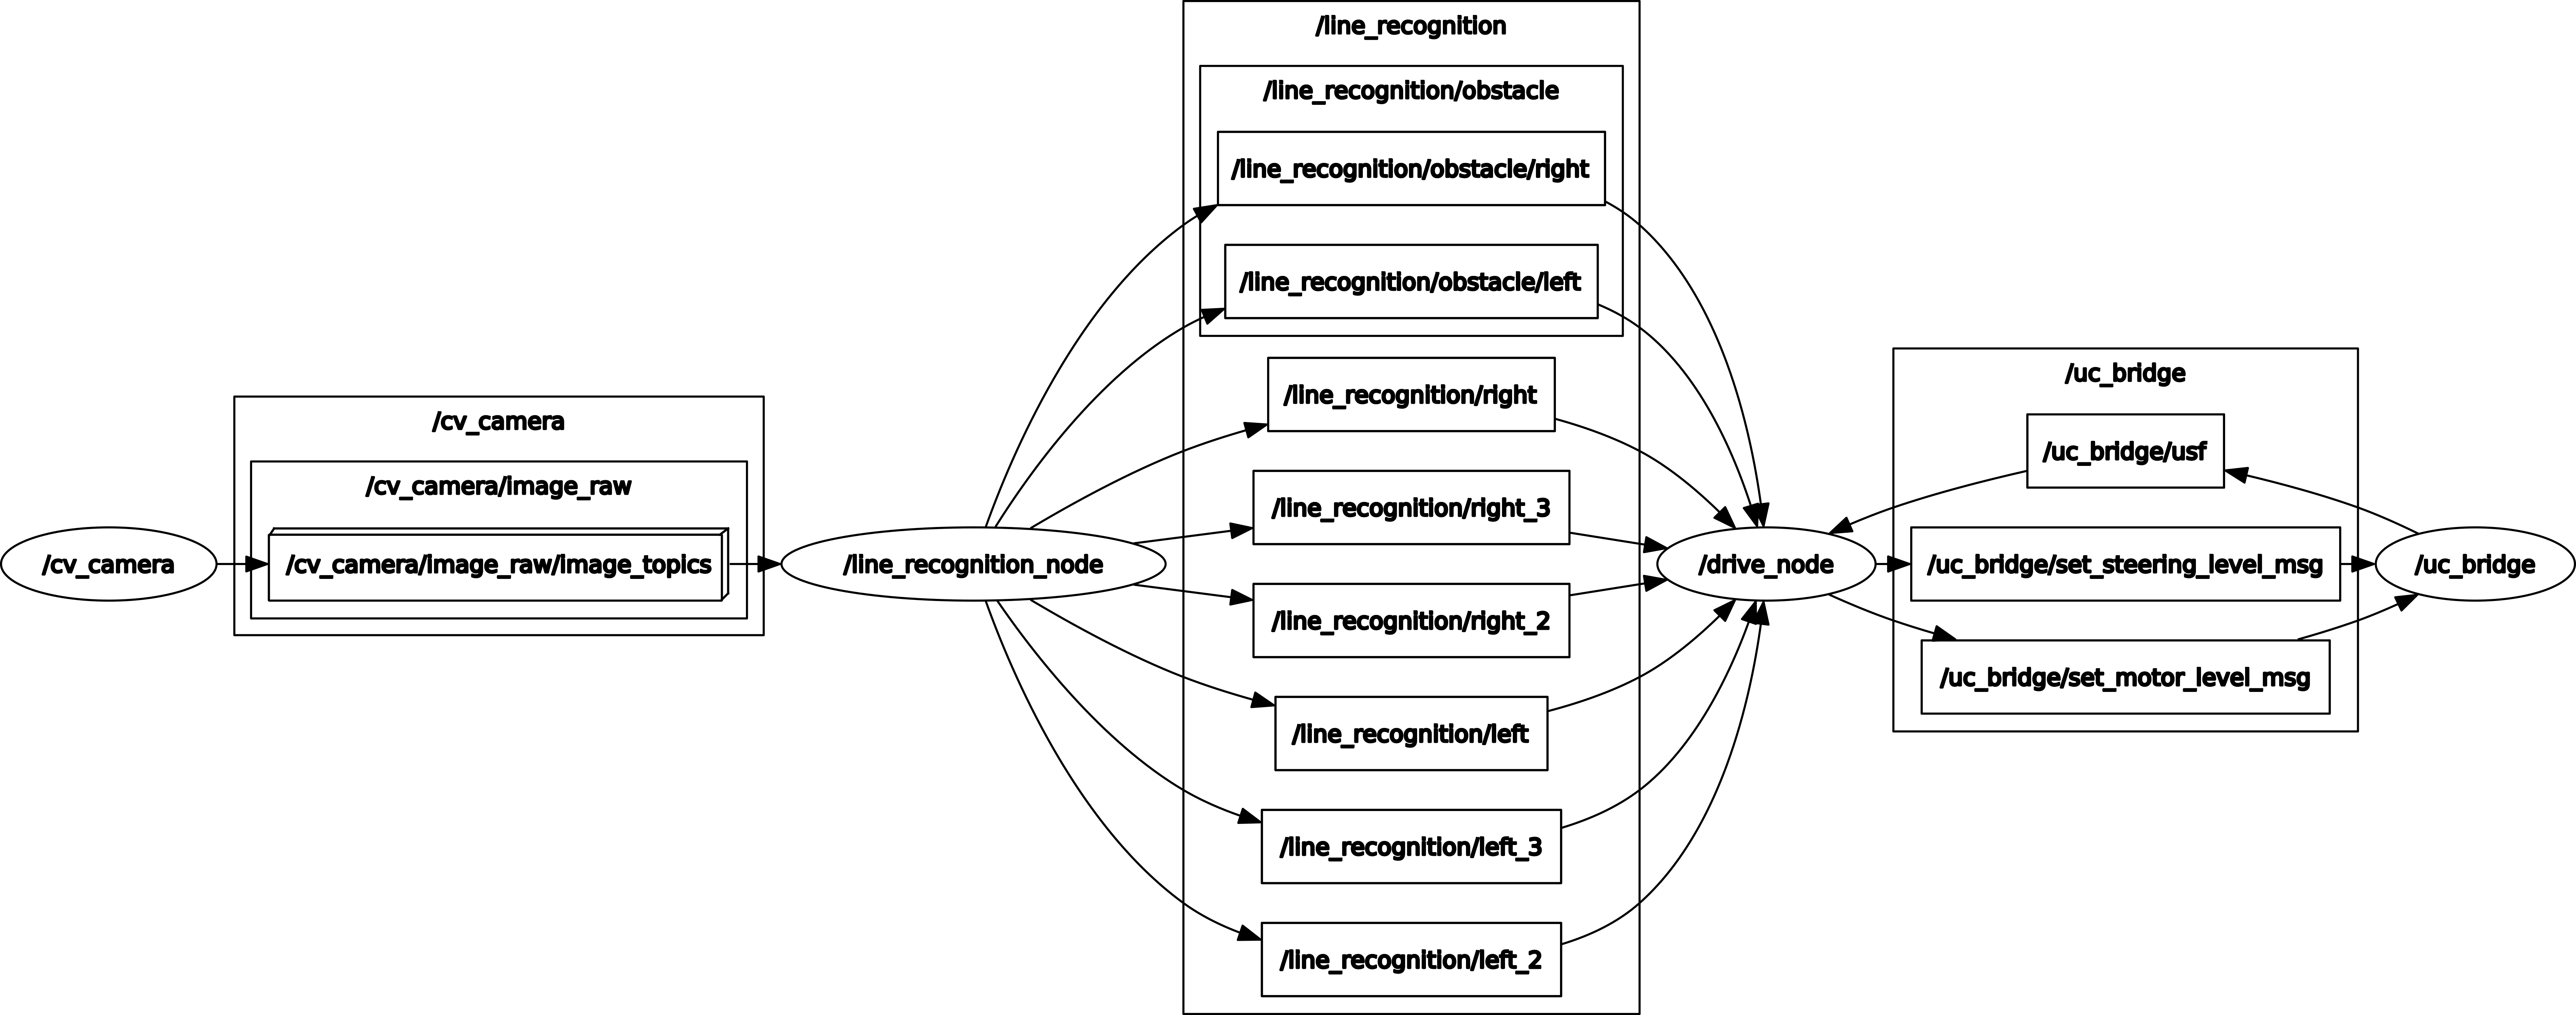
\includegraphics[width=\textwidth]{images/rosgraph.png}
	\caption{Nodes und Topics der Implementierung}
\end{figure}
\label{graph}

\subsection{Bildverarbeitung und Erkennung von Fahrspuren}
\label{sec:spurerkennung}
Zur Bilderzeugung konnte zwischen zwei Kamerasystemen gewählt werden: Einer Kinect Kamera sowie einer Weitwinkel Webcam. Die Entscheidung fiel auf die Weitwinkel Webcam, da sich diese aufgrund ihrer Weitwinkel- und Farbdarstellungseigenschaft und den in \autoref{cha:Probleme} genannten Problemen der Kinect Kamera als besser geeignet herausstellte. 

Die mittels OpenCV eingelesenen Kamerabilder werden durch die Natur der Kameraposition in Zentralperspektive aufgezeichnet. Diese Art der Projektion eignet sich aufgrund des vorhandenen Fluchtpunktes nicht für die benötigte Bildverarbeitung, weshalb eine Transformation in Vogelperspektive durchgeführt wird, welche die Problematik des Fluchtpunktes beseitigt.

Zur Erkennung der Fahrspuren wurden die Farbwerte der grünen äußeren Fahrbahnmarkierungen ermittelt. Mithilfe dieser Farbwerte kann ein Graustufenbild erzeugt werden, welches die Übereinstimmung mit dem vorgegebenen Farbwert repräsentiert. Je mehr der Farbpixel des Originalbildes mit dem verglichenen Farbwert übereinstimmt, desto heller erscheint der Pixel an seiner Stelle im Graustufenbild. Um die Orientierung in diesem sicherzustellen, werden drei Marker in äquidistanter Höhe auf die rechte und linke Linie gesetzt (siehe Abbildung 4.2). Der Algorithmus zur Positionierung der Marker sucht dabei zeilenweise im Bild nach aufeinanderfolgenden hellen Pixeln und addiert die Helligkeit dieser Pixel auf. Übersteigt diese Summe einen Schwellwert, so wird diese Stelle mit einem Marker versehen.

\begin{figure}[ht]
	\centering
	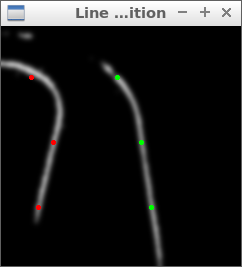
\includegraphics[width=0.35\textwidth]{images/isnt_straight_original.png}
	\caption{Fahrspur mit Markern}
\end{figure}
\label{Bild von Fahrspuren}

\subsection{Erkennung von Kurven und Geraden}
\label{sec:kurvenerkennung}
Um das Fahrverhalten besser anpassen zu können, fiel die Entscheidung darauf Fahrmodi zu erstellen, welche unterschiedliche Reglerparameter besitzen. Um diese Fahrzustände korrekt erkennen zu können ist es von Nöten zwischen Geraden, Kurven, Kurvenein- und Kurvenausfahrten zu unterscheiden.

Um eine Kurve zu erkennen, werden die drei gesetzten Marker jener Seite betrachtet, an welcher sich das Fahrzeug gerade orientiert. Da sich diese in gleichem vertikalen Abstand zu einander befinden wird lediglich der horizontale Abstand betrachtet. Zuerst wird hierfür der vertikale Abstand zwischen dem unteren sowie dem mittleren Marker ermittelt. Dieses Verfahren wird mit dem oberen und dem mittleren wiederholt. Übersteigt die Differenz der beiden ermittelten Abstandswerte einen Schwellwert, so liegt eine Kurve vor. Abbildung 4.3 zeigt eine solche Situation.

Um nun auch Kurvenein- und Kurvenausfahrten erkennen zu können, wurde ein Puffer implementiert, welcher aus vorherigem und aktuellem Kurvenerkennungswert ermitteln kann in welcher Umgebungssituation sich das Fahrzeug befindet. Des Weiteren dient der Puffer als eine Hysterese, welche ein Flackern der Fahrzustände vermeidet.

\begin{figure}[ht]
	\centering
	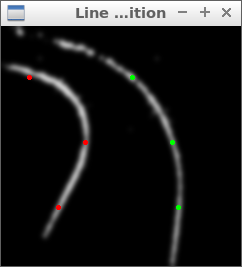
\includegraphics[width=0.35\textwidth]{images/curve_bw.png}
	\caption{Kurveneinfahrt mit Makern}
\end{figure}
\label{Bild von Kurve}

\subsection{Erkennung von Hindernissen}
\label{sec:hinderniserkennung}
Wie auch die Fahrspurerkennung, basiert die Hinderniserkennung auf der Filterung der Kamerabilder auf eine spezielle Farbe. Aus diesem Grund wurden die Hinderniswürfel, um sie vom Rest der Kulisse unterscheiden zu können mit orangefarbenem Klebeband versehen. Um sicher zu gehen, dass nicht fälschlicherweise ein Hindernis erkannt wird, wird ein ähnlicher Algorithmus wie bei der Fahrspurerkennung angewandt. Des Weiteren wird ein Hindernis nur als solches erkannt, wenn zwei vertikale Linien nebeneinander erkannt werden, wie es bei den Hinderniswürfeln der Fall ist. 
\begin{figure}[h]
	\centering
	\begin{subfigure}{0.45\textwidth}
		\centering
		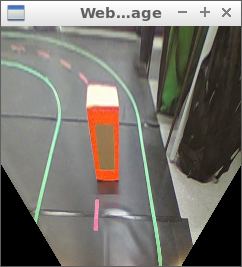
\includegraphics[width=0.9\textwidth]{images/obstacle_original.png}
		\caption{Transformiertes Farbbild}
	\end{subfigure}
	\begin{subfigure}{0.45\textwidth}
		\centering
		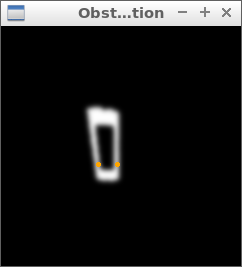
\includegraphics[width=0.9\textwidth]{images/obstacle_alone_bw.png}
		\caption{Hindernis nach Filterung}
	\end{subfigure}
	\begin{subfigure}{0.45\textwidth}
		\centering
		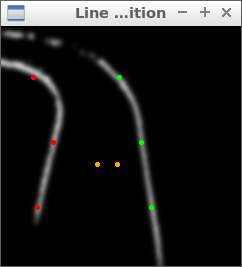
\includegraphics[width=0.9\textwidth]{images/obstacle_bw.png}
		\caption{Markiertes Hindernis}
	\end{subfigure}
	\caption{Fahrspur mit Hindernis}
	\label{Bild von Hindernis}
\end{figure}
Prinzipiell wäre es somit auch möglich andere Gegenstände in die Fahrspur zu stellen, solange diese zwei vertikale orangefarbene Streifen besitzen. Dies wurde mit einem auf einer Spur fahrenden Fahrzeug einer anderen Gruppe erfolgreich getestet. Abbildung 4.4 zeigt die verschiedenen Phasen der Hinderniserkennung.
\subsubsection{Kollisionsvermeidung}
\label{sec:kollision}
Um in allen Fahrsituationen eine Beschädigung des Fahrzeugs zu vermeiden, wird eine Kollisionsvermeidung eingesetzt. Diese verhindert unabhängig von Fahrspuren oder erkannten Hindernissen, dass es im Fahrbetrieb zu einem Zusammenstoß mit anderen Gegenständen oder der Wand kommt. Hierzu werden die Daten des vorderen Ultraschallsensors ausgewertet, der einen ungefähren Abstandswert zum nächstgelegenen Gegenstand liefert.

Um aus dem fehlerbehafteten Signal verwertbare Daten zu erhalten werden die Werte des Sensors geglättet. Dies geschieht indem die letzten 20 Sensorwerte gemittelt werden. Liegt der Durchschnitt unter einem Schwellwert, wird der Motor angehalten. Als praxistauglicher Wert hat sich 0.35 erwiesen, also ein Abstand von 35 Zentimetern.

Ein besonderes Problem ergibt sich aus der Tatsache, dass die Werte des Sensors in unregelmäßigen Abständen kurzzeitig auf den Wert Null springen. Dies entspräche einem Gegenstand direkt vor dem Sensor, was schon alleine aufgrund der Fahrzeuggeometrie nicht plausibel ist. Diese Werte müssen daher von der Auswertung ausgenommen werden.

\lstinputlisting[firstline=159, lastline=187, caption={Codeausschnitt zu Collision Detection}, label={code:collision}]{../../drive/src/drive_node.cpp}

\subsubsection{Regelungskonzept und Spurhaltung}
\label{sec:wallfollower}
Nach umfangreichen Tests zu Beginn des Projekts wurde ein strukturvariabler Regelungsansatz mit PD-Reglern gewählt. Eine strukturvariable Regelung lässt sich vor Allem dann sinnvoll einsetzen, wenn zwischen wenigen bekannten Arbeitspunkten umgeschaltet werden muss. Die Rennstrecke des Projektseminars Echtzeitsysteme lässt sich in Kurven- und Geradenabschnitte aufteilen. Aufgrund der hohen Nichtlinearität der Lenkungsmechanik (insbesondere Lose, Haftreibung, Gleitreibung) lässt sich mit einem einzigen PD-Regler kein zufriedenstellendes Regelverhalten in allen Fahrsituationen erzielen. Eine stationäre Genauigkeit ist in diesem Fall zur Spurhaltung im Übrigen nicht erforderlich, solange die bleibende Regelabweichung in der Praxis so klein ist, dass alle Fahrsituationen der Rennstrecke ohne Linienüberschreitung gefahren werden können. Mit mehreren gut eingestellten PD-Reglern lässt sich diese Anforderung erfüllen.

Die Bildverarbeitung liefert die Positionsdaten aller Markierungslinien, die im Bildausschnitt der Kamera erfasst werden. Da die Position der Kamera auf dem Fahrzeug sich nicht ändert, kann ein fester Sollwert für den Abstand zu diesen Linien vorgegeben werden. Es muss zur Berechnung der Regelabweichung lediglich bekannt sein, ob das Fahrzeug sich an der rechten oder an der linken Fahrbahnbegrenzung orientieren soll. Näheres hierzu in \autoref{sec:fahrsituationen}.


\subsubsection{Implementierung des PD-Reglers}
\label{sec:pdregler}
Die Berechnung der Lenkwinkelregelung erfolgt in mehreren Schritten. Zunächst wird aus den situationsabhängigen Reglerparametern sowie Führungsgröße und aktueller Position eine Stellgröße berechnet. Der differentielle Anteil des PD-Reglers greift hierbei auf den aktuellen und vorherigen Wert der Regelabweichung, sowie die verstrichene Zeitdauer seit der letzten Berechnung zu.

\lstinputlisting[firstline=638, lastline=642, caption={Codeausschnitt zur Implementierung des PD-Reglers}, label={code:pdregler}]{../../drive/src/drive_node.cpp}

Anschließend erfolgt eine Begrenzung der Stellgröße. Die Hardware erlaubt Lenkwinkel im Bereich -800....+800. Um Beschädigungen zu vermeiden wird der maximale Lenkwinkel softwareseitig auf -700....+700 begrenzt. Bei höheren Werten kommt es zu einem Blockieren des Lenkgetriebes.

Um ein ruhiges Lenkverhalten zu erreichen, werden die Ausgangswerte des Reglers zum Schluss geglättet. Dazu wird ein gewichteter Mittelwert der letzten Stellgrößen gebildet. Die Gewichtung erfolgt in Abhängigkeit des zeitlichen Verlaufs. Dabei hat der zuletzt berechnete Wert das größte Gewicht, ein 0,3 Sekunden zurückliegender Wert hingegen nur das halbe Gewicht. Der gewichtete Mittelwert erzeugt ein ruhiges Regelverhalten, ohne jedoch die Regelung zu stark zu verzögern.

\lstinputlisting[firstline=661, lastline=682, caption={Codeausschnitt zu Begrenzung und Glättung der Stellgrößen}, label={code:glaettung}]{../../drive/src/drive_node.cpp}

\subsubsection{Implementierung verschiedener Fahrsituationen}
\label{sec:fahrsituationen}
Das Konzept sieht die Aufteilung der zu fahrenden Strecke in vier wiederkehrende Fahrsituationen vor:

\begin{itemize}
	\item Geradeausfahrt
	\item Kurvenfahrt
	\item Übergang von Geraden- zu Kurvenfahrt
	\item Übergang von Kurven- zu Geradenfahrt
\end{itemize}

Je nach Situation wird zwischen einem Regler für Geradeausfahrt und einem Regler für Kurvenfahrt umgeschaltet. Die Übergangszustände dienen lediglich der stufenweisen Geschwindigkeitsanpassung beim Wechsel zwischen den beiden Streckenabschnitten. Die Umschaltung zwischen den verschiedenen Reglern erfolgt in Abhängigkeit vom gewählten Fahrmodus (siehe \autoref{sec:fahrmodi}).

Der Regler für die Geradeausfahrt zeichnet sich durch eine deutlich niedrigere Gewichtung von P- und D-Anteil aus, während der Regler für die Kurvenabschnitte mit einer hohen Verstärkung eher aggressiv abgestimmt ist.


\subsubsection{Einleitung eines Spurwechsels}
\label{sec:spurwechsel}
Die Implementierung eines Spurwechsels eröffnet vielfältige Möglichkeiten. Während ein Spurwechsel auf geraden Abschnitten der Strecke unproblematisch ist, kann es im Zusammenhang mit Kurven zu Problemen kommen. Wird eine Kurve auf der äußeren Spur durchfahren, so ist während der Kurvenfahrt grundsätzlich kein Wechsel auf die innere Spur möglich. Die konstruktive Begrenzung des Lenkwinkels wird durch die Kurvenfahrt schon komplett ausgenutzt, sodass kein Spielraum für ein Ausweichen nach innen mehr bleibt. Weniger problematisch ist das Ausweichen von der inneren auf die äußere Spur während einer Kurvenfahrt.

Auf der Rennstrecke des Projektseminars gibt es nur zwei Varianten eines Spurwechsels: von der rechten auf die linke Spur, und von der linken auf die rechte Spur. Grundsätzlich können diese Wechsel vorgenommen werden, indem der Regler-Sollwert auf den jeweils anderen Fahrbahnrand gesetzt wird. Dazu muss jedoch zunächst sichergestellt werden, dass sich überhaupt beide Fahrbahnmarkierungen im Sichtfeld der Kamera befinden. Wird ein Spurwechsel veranlasst, lenkt das Fahrzeug daher zunächst für eine kurze Zeit mit vollem Einschlag in die gewünschte Richtung. Nun kann davon ausgegangen werden, dass beide Fahrspuren erfasst werden. Um zügig eine gute Position in der neuen Spur zu erreichen, wird anschließend auf einen sehr hart abgestimmten Regler geschaltet, bevor wieder die normalen Kurven- und Geradenregler zum Einsatz kommen. Das Fahrzeug ist dann wieder bereit um jederzeit auf die andere Spur zu wechseln.


\subsubsection{Fahrmodi und Wettbewerb}
\label{sec:fahrmodi}
Im Rahmen dieses Projektseminars sind zwei Aufgaben zu erfüllen: das Absolvieren einer kompletten Runde in möglichst geringer Zeit, und die Hinderniserkennung mit Spurwechsel bei möglichst wenigen Linienübertritten. Um beide Aufgaben möglichst gut zu lösen werden zwei verschiedene Fahrmodi implementiert, die sich durch die Fahrgeschwindigkeit und die Kriterien zur Wahl der Fahrspur unterscheiden.

\paragraph{Fahrmodus 1: Rundenzeit}

Im ersten Fahrmodus liegt die Herausforderung in der Minimierung der Rundenzeiten. In diesem Modus wird ohne Hindernisse auf der Strecke gefahren, daher ist die Hinderniserkennung abgeschaltet. Das Fahrzeug fährt mit variabler Geschwindigkeit: auf längeren Geradenabschnitten kann mit deutlich höherer Geschwindigkeit gefahren werden als im Bereich von Kurven. Das Fahrzeug orientiert sich in diesem Modus stets an der äußeren Fahrbahnmarkierung, also der Markierung mit dem größeren Kurvenradius. Dies dient der Erhöhung der Stabilität in Kurven.

\paragraph{Fahrmodus 2: Hinderniserkennung und Spurwechsel}

In diesem Modus spielt die Fahrgeschwindigkeit eine untergeordnete Rolle, weshalb sie auf einen konstanten und relativ niedrigen Wert gesetzt wird. Zunächst orientiert sich das Fahrzeug am rechten oder linken Fahrbahnrand und folgt der Spur. Solange sich kein Hindernis auf der Strecke befindet, wird dieser Zustand beibehalten. 

Ein Spurwechsel setzt voraus, dass dem Fahrzeug die eigene Position auf der Fahrbahn bekannt ist. Da dem Fahrzeug vorgegeben wird auf welcher Fahrspur es fahren soll, und die Regler ein schnelles Regelverhalten besitzen, kann im Allgemeinen davon ausgegangen werden, dass sich das Fahrzeug auf der vorgegebenen Fahrspur befindet.

Sobald ein Hindernis in das Sichtfeld der Kamera eintritt liefert die Bildverarbeitung dessen Koordinaten. Da auch die Koordinaten der beiden Fahrspuren bekannt sind, kann aus den Daten ermittelt werden, ob sich das Hindernis auf der aktuellen Fahrspur des Autos befindet. Befindet sich das Hindernis auf der eigenen Fahrspur, wird rechtzeitig ein Spurwechsel veranlasst. Andernfalls wird das Hindernis ignoriert und die Fahrt fortgesetzt.

Der Spurwechsel wird durch die Erkennung eines Hindernisses eingeleitet. Die Bildverarbeitung liefert dabei die Positionen des rechten und linken Randes eines Hindernisses, sodass neben der Position auch dessen Breite bekannt ist (siehe \autoref{sec:hinderniserkennung}). Für den Spurwechsel entscheidend ist die Frage, ob sich das erkannte Hindernis überhaupt auf der gleichen Fahrspur wie das Fahrzeug befindet. Ist das nicht der Fall, stellt es kein Hindernis dar und kann ignoriert werden.
